\section{Definitions for shortest paths and shortest k-paths}

In this section we will go through formal definitions and properties of
shortest paths and shortest $k$-paths. To precisely define these we need
understand several other concepts of geometry in the plane and graph theory. \\

We start with a trivial definition which we will expand upon.

\begin{mydef}\textbf{Path:}
Given a plane encapsulated by a polygon $\mathcal{P}$, let $s$ and $t$ be two
	points in the plane. We define a path between $s$ and $t$ to be a set of
	vertices and edges which forms a connection from $s$ to $t$.
\end{mydef}

Its trivial to see that a path with a minimum length in the case where $s$ and $t$
are the only entities in the plane will be $\overline{st}$. But we can imagine the
space being occupied not only by two points $s$ and $t$, but also with a set of 
polygons in which a path cannot pass through. We call such polygons obstacles and
we assume through out the rest of this thesis that these obstacles will be 
simple polygons. Since we will represent these with graphs we give a definition of 
simples graphs.

\begin{mydef}\textbf{Simple Graph:}
  A graph is simple if it has no loops and no two of its links join the same pair
  of vertices.
\end{mydef}

Now we might be in a situation where the path with minimum length between two point 
$s$ and $t$ isn't just $\overline{st}$ due to obstacles being placed in the way. We 
further define what space we can create our path in, and which we cannot.

\begin{mydef} 
	\textbf{Free space:}\\ 
	Let $\mathcal{O}=\{O_1,O_2,...,O_k\}$ be a
	family of simple polygons which will act as obstacles in the interior of an
	encapsulating polygon $\mathcal{P}$. We define the free space to be
	$\mathcal{FS}=\mathcal{P}\setminus\mathcal{O}$, that is the plane of the
	encapsulating polygon minus the interiors of all obstacle polygons.
\end{mydef}

The algorithms that we will be examining will mostly need the obstacles to be 
convex, which are defined as follows: 

\begin{mydef}
	\textbf{Convex Polygons:} \\ 
	A convex polygon is a simple polygon (not self-intersecting) in which no
	line segment between two points on the boundary ever goes outside the
	polygon. In a convex polygon, all interior angles are less than or equal to
	180 degrees, while in a strictly convex polygon all interior angles are
	strictly less than 180 degrees.
	\cite{Bisector-collinearity-convexPoly} 
\end{mydef}

We are only allowed to make paths between $s$ and $t$ in the free space, which we 
will denote as legal paths.

\begin{mydef}
	\textbf{Legal Path:}\\ 
	We define a path between to vertices to be
	legal if it lie entirely in the free space. That is a legal path is disjoint
	from the interiors of all potential obstacle polygons in the plane.
\end{mydef}

Now we are ready to define out legal shortest path between our two points $s$ and 
$t$

\begin{mydef}
	\textbf{Euclidian shortest path:}\\ 
	The legal path of minimum total length connecting the two endpoints is a 
    shortest path.  
\end{mydef}

We define a path which is not legal to be violating, or having a number of
violations, equal to the number of obstacles in which the path will pass
through. We will not only deal with shortest paths which have no violations,
but also shortest path which allow up to $k$ violations.

\begin{mydef}
	\textbf{Shortest k-path}
	The path of minimum total length which violates at most $k$ obstacles.
\end{mydef}

Through out this thesis we will use use the notation of $\pi(s,t)$ to denote the 
shortest paths connecting two points $s$ and $t$ in the case where no obstacle 
violation is allowed. The length of any path in	$\pi(s,t)$ is the shortest path 
distance between $s$ and $t$, denoted $d(p,q)$. If the shortest path between $s$ 
and $t$ is the line segment $\overline{p,q}$, then $p$ and $q$ are said to be 
visible. 

\begin{mydef}
	\textbf{Visibility between points:}
    We define two points $s$ and $t$ to be visible to each other if $s$ and $t$ are 
    connectible with the path $\overline{st}$ which is either legal, or in the case 
    of violations have less that the allowed $k$ violations.
\end{mydef}

The notion of shortest path distance between two sets of points $X$ and $Y$ is 
denoted as $d(X,Y)$ and is the minimum $d(x,y)$ over all pairs of points $x\in X$ 
and $y \in Y$. \cite{HershbergerS99} \\

We call a path violating of at most $k$ obstacles a \textit{$k$-path}, generalizing 
on the traditional obstacle-free path, which is a 0-path. We use the notation of 
$\pi_k(p)$ to be the shortest path in this case where the path can pass through up 
to $k$ obstacles from a \textit{fixed source} $s$ to the point $p$. When reasoning 
about a path with exactly $k$ crossing we denote this as an $(=k)$-path. And 
equally we use $d_k(p)$ to denote the length of the shortest path from the fixed 
source $s$ in the case of up to $k$ obstacle violations. The reason we use a 
separate notation in the case of obstacle violation is that shortest 0-path 
problem with origination at a common source point $s$ cannot intersect, by the 
triangle inequality\cite{HershbergerKS17}\footnote{this will be proven later in 
the thesis}.

\begin{mydef}
	\textbf{Triangle Inequality:} \\ 
	Let $A$ and $B$ be points in a $\mathbb{R}^n$ space and let $|AB|$ denote
	the distance between $A$ and $B$.  Then the triangle inequality states that
	for three points $A,B,C\in\mathbb{R}^n$ \cite{metricspaceandpoints}
	$$|AB|\leq|AC|+|BC|$$
\end{mydef} 
\begin{figure}[H] 
	\centering
	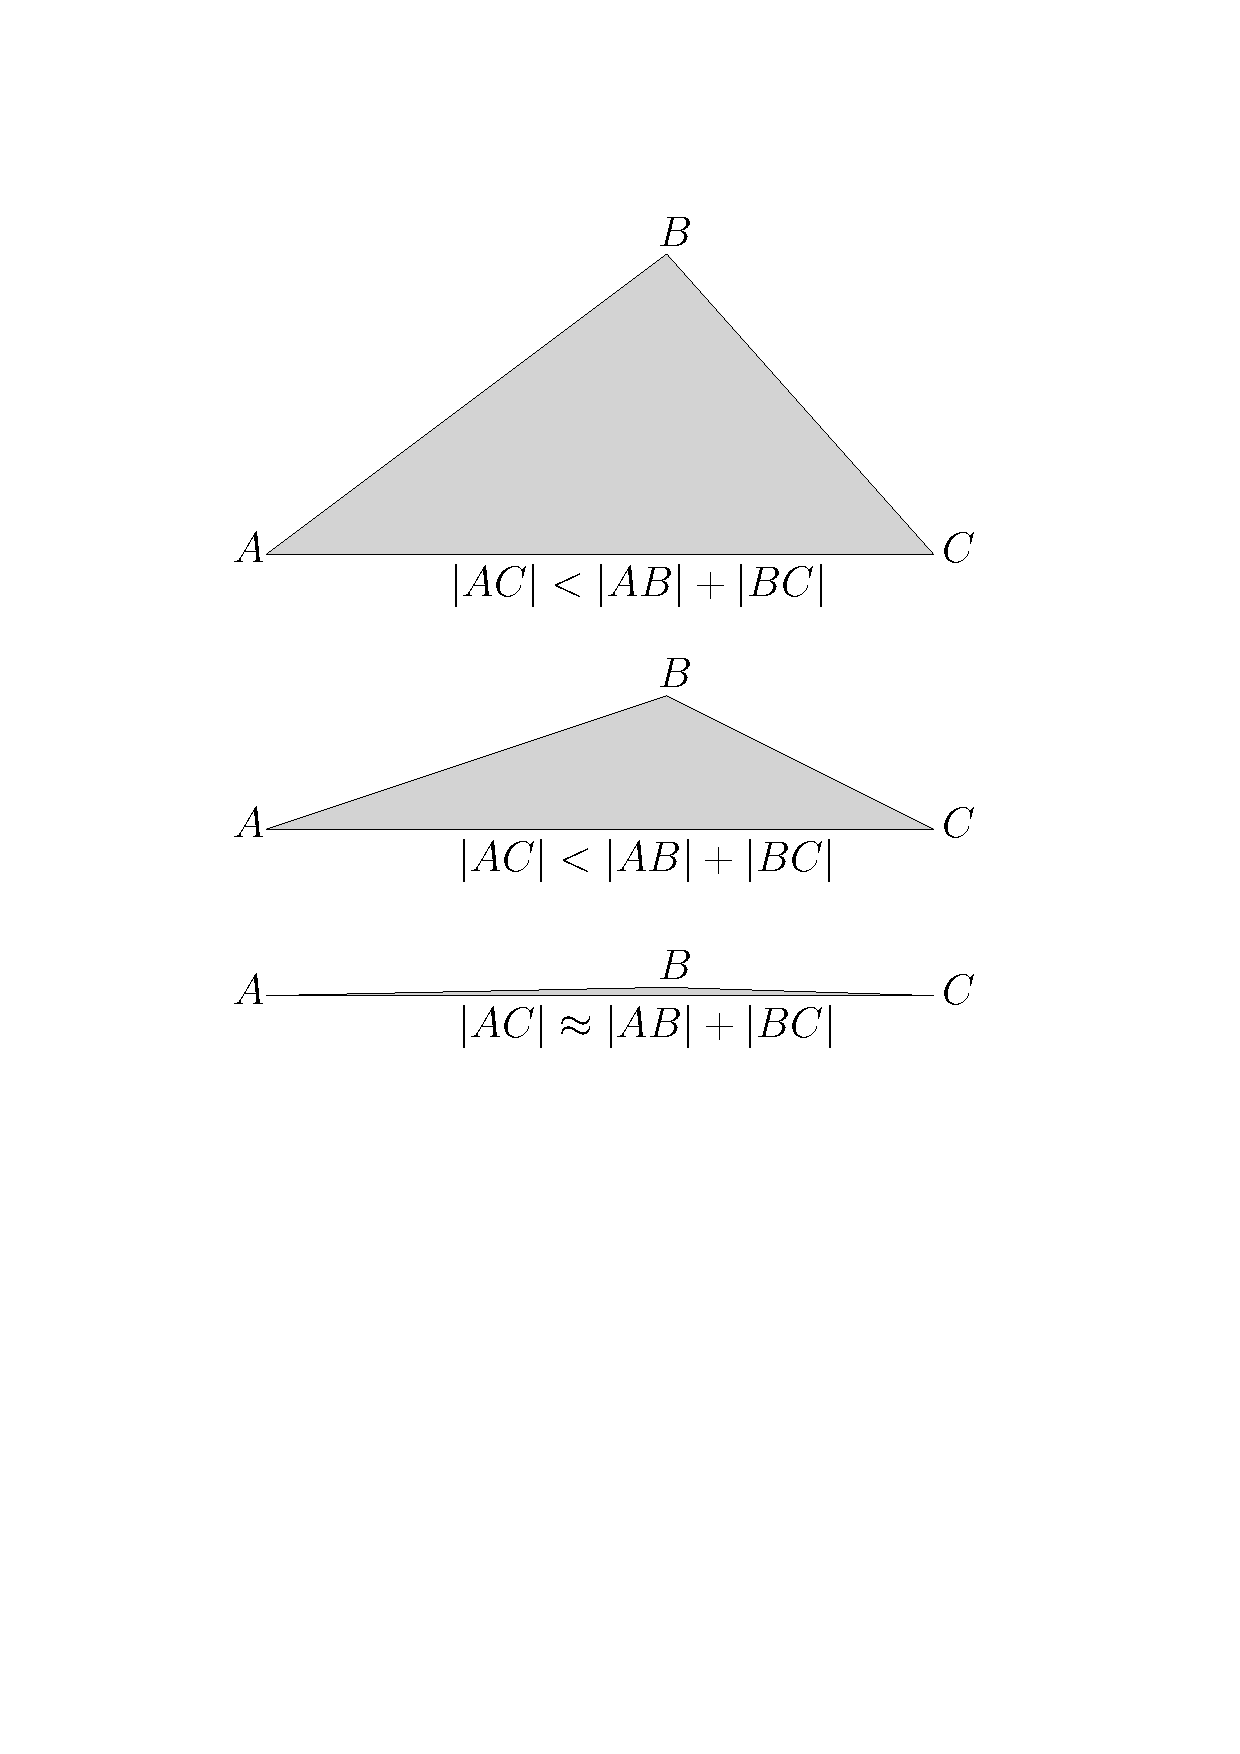
\includegraphics[width=5cm]{pictures/TriangularInequality.pdf}
	\caption{Triangular Inequality approaching equality}
	\label{fig:TriangularInequality} 
\end{figure}


\section{Shortest path map}

\section{Shortest k path map}

\section{Differences between $SPM$ and $SPM_k$}

\subsection{Given slack when going to k violations}